\documentclass{article}

\usepackage[%
    left=0.5in,%
    right=0.5in,%
    top=0.5in,%
    bottom=0.5in,%
]{geometry}%
\usepackage{minitoc}
\usepackage{multicol}
\usepackage{graphicx}
\usepackage{fixltx2e}
\usepackage{listings}
\usepackage{color}
\usepackage{hyperref}
    \hypersetup{ colorlinks = true, linkcolor = blue }
\usepackage{blindtext}
\definecolor{lightgray}{gray}{0.9}
\graphicspath{ {./} }

\newcommand{\inlinecode}[2]{\colorbox{lightgray}{\lstinline
[language=#1]$#2$}}
\newcommand{\worddef}[1]{\hyperref[sec:reference]{\textit{#1}}}

\begin{document}

\section{Definition of a graph}
\begin{flushleft}
A graph is a set of nodes, or vertices, connected by edges
\end{flushleft}

\section{Applications}
\begin{itemize}
	\item Networks (e.g., of computers or roads)
	\item Flow charts
	\item Tasks in some project (some of which should be completed before others), so edges correspond to prerequisites 
	\item States of an automaton / program
\end{itemize}

\section{Directed and Undirected}
\begin{itemize}
	\item undirected – edges don’t have direction (relationship goes both ways)
	\item directed (digraph) – edges have direction (relationship flow has to be defined)
\end{itemize}
\begin{flushleft}
	Undirected graphs can be represented as directed graphs where for each edge (X,Y) there is a corresponding edge (Y,X).
\end{flushleft}
\begin{center}
	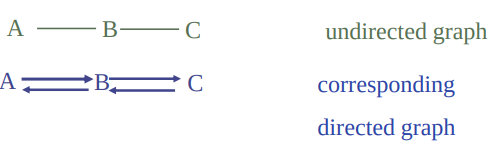
\includegraphics[scale=0.5]{graph_egzample_1.png}
\end{center}

\section{Notation}
\begin{itemize}
	\item Set $V$ of vertices (nodes)
	\item Set $E$ of edges $E \subseteq V \times V$
\end{itemize}
\begin{center}
	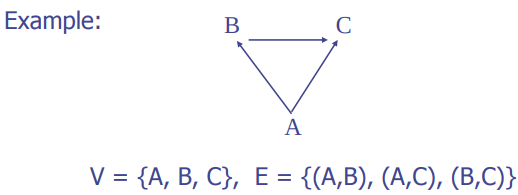
\includegraphics[scale=0.5]{graph_example_2.png}
\end{center}
\begin{itemize}
	\item Node B is \textit{adjacent} to A if there is an edge from A to B. ($A \rightarrow B$)
	\item A \textit{path} from A to B is a sequence of vertices where each vertex points to the second one 
	\item A vertex B is \textit{reachable} from A if there is a path from A to B
	\item A \textit{cycle} is a path from a vertex to itself
	\item Graph is \textit{acyclic} if it does not have cycles
	\item An \textbf{undirected} graph is \textit{connected} if there is a path between every pair of vertices
	\item For a directed graph:
	\begin{itemize}
		\item It is \textit{weakly connected} if the corresponding \textit{undirected graph} is \textbf{connected} (i.e. if we permit traversal of edges in any direction)
		\item It is \textit{strongly connected} if for every ordered pair (v1,v2) of vertices, there is a path that respects the directions of the edges, and that goes from v1 to v2. Note need paths from v1 to v2, and also v2 to v1.
	\end{itemize}
\end{itemize}

\section{Common graph problems}
\begin{itemize}
	\item Searching a graph for a vertex
	\item Searching a graph for an edge
	\item Finding a path in the graph (from one vertex to another)
	\item Finding the shortest path between two vertices
	\item Cycle detection
\end{itemize}
Implementation
\begin{itemize}
	\item \textbf{static} indexed data structure: \textit{Adjacency Matrix}
	\item \textbf{dynamic} data structure \textit{Adjacency Lists}
\end{itemize}

\section{Static Implementation: Adjacency Matrix}
\begin{itemize}
	\item Store node in an array: each node is associated with an integer (array index inside 2D grid)
	\item Represent information about the edges using a two dimensional array, 
		where \inlinecode{C}{array[i][j] == 1} iff there is an edge from node with index \texttt{i} to the node with index \texttt{j}.
\end{itemize}
\begin{center}
	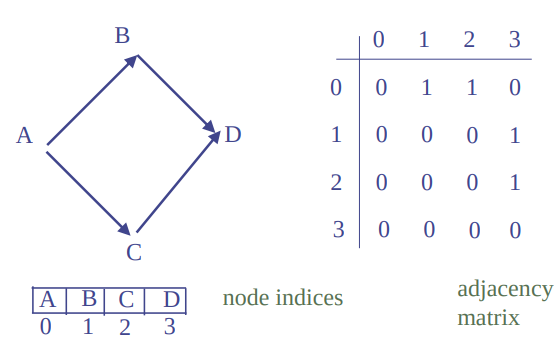
\includegraphics[scale=0.5]{adjacency_matrix.png}
\end{center}
\begin{flushleft}
For weighted graphs, place weights in the matrix if there is no edge we use a value which can’t be confused with a weight, e.g., \texttt{-1} or \verb!Integer.MAX_VALUE!
\end{flushleft}

\subsection{Disadvantages}
\begin{itemize}
	\item Sparse graphs with few edges for number that are possible result in many zero entries in adjacency matrix
 	\item This \textbf{wastes space} and makes many algorithms \textbf{less efficient}  e.g., to find nodes adjacent to a given node, we have to iterate through the whole row even if there are few 1s there.
 	\item Also, if the number of nodes in the graph may change, matrix representation is too b  especially if we \textbf{don’t know} the maximal size of the graph.
\end{itemize}

\section{Adjacency List}
\begin{itemize}
	\item For every vertex, keep a \textbf{list} of adjacent vertices.
	\item Keep a list of vertices, or keep vertices in a Map (e.g. HashMap) as keys and lists of adjacent vertices as values. (The best choice depends on what the graph algorithm needs to do.)
	\item Example: A - key, "B, C" - value(list of nodes that A points to) $ A \rightarrow B, C$
\end{itemize}

\pagebreak
\section*{Reference section} \label{sec:reference}
\begin{description}
	\item[placeholder] \hfill \\
\end{description}
\end{document}
